\subsection{QuizziPedia::Back-End::App::Controllers::Users}
\subsubsection{Informazioni generali}
\label{QuizziPedia::Back-End::App::Controllers::Users}
\begin{figure}[ht]
	\centering
	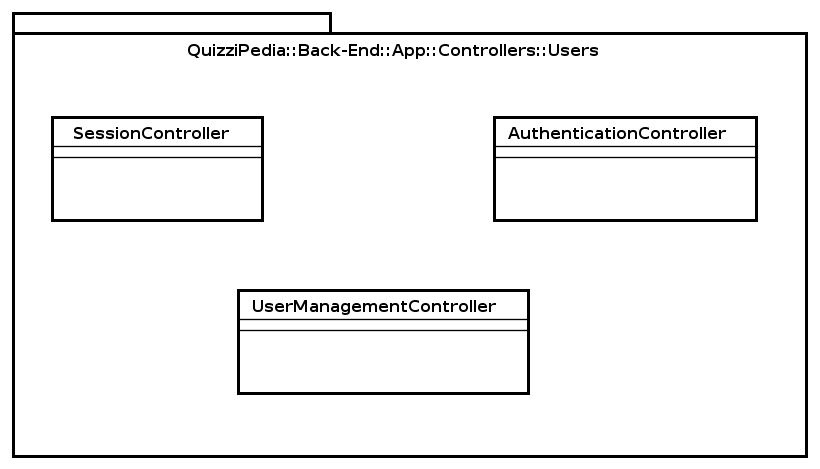
\includegraphics[scale=0.45]{UML/Package/QuizziPedia_Back-End_App_Controllers_Users.png}
	\caption{QuizziPedia::Back-End::App::Controllers::Users}
\end{figure}
\FloatBarrier
\begin{itemize}
	\item 
	\textbf{Descrizione}:\\
	\textit{Package\ped{G}} contenente i controllers relativi alla gestione dell'autenticazione e dei dati dell'utente;
	\item
	\textbf{Padre}:\\
	\texttt{Controllers}
\end{itemize}	
\subsubsection{Classi}
\paragraph{QuizziPedia::Back-End::App::Controllers::Users::AuthenticationController}
\label{QuizziPedia::Back-End::App::Controllers::Users::AuthenticationController}
\begin{figure}[ht]
	\centering
	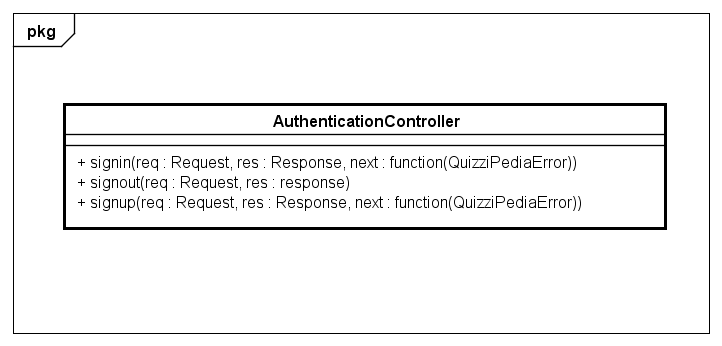
\includegraphics[scale=0.45]{UML/Classi/Back-End/QuizziPedia_Back-End_App_Controllers_Users_AuthenticationController.png}
	\caption{QuizziPedia::Back-End::App::Controllers::Users::AuthenticationController}
\end{figure}
\FloatBarrier
\begin{itemize}
	\item 
	\textbf{Descrizione}:\\
	Classe che si occupa della registrazione e dell'autenticazione dell'utente nel sistema. È un componente ConcreteHandler del design pattern \textit{Chain of responsibility\ped{G}}. Risulta essere il componente che eventualmente esegue la richiesta del client attraverso \textit{Passport\ped{G}};
	\item
	\textbf{Utilizzo}:\\
	Viene utilizzata per implementare le funzionalità necessarie a gestire le richieste \textit{REST\ped{G}} legate alla registrazione e all'autenticazione dell'utente;
	\item
	\textbf{Relazioni con altre classi}:
	\begin{itemize}
		\item
		IN \texttt{UserController} \\
		Classe che raggruppa attraverso require i vari controllers responsabili delle operazioni legate alla gestione degli utenti. Si è scelto di predisporre questo raggruppamento per facilitare l'introduzione di nuove funzionalità legate alla gestione degli utenti;
		\item
		OUT \texttt{Session} \\
		Classe che gestisce la sessione utente dell'applicazione. Non sono stati modellati attributi e metodi di questa classe in quanto viene inizializzata da \textit{Express\ped{G}} ed utilizzata da \textit{Passport\ped{G}} attraverso funzionalità interne ai due \textit{middleware\ped{G}};
		\item
		OUT \texttt{UserModel} \\
		Classe che modella la creazione e la gestione dei dati utente.
	\end{itemize}
	\item
	\textbf{Metodi}:
	\begin{itemize}
		\item
		\texttt{+ signin(req: Request, res: Response, next: function(QuzziPediaError))} \\
		Esegue l'autenticazione attraverso \textit{Passport\ped{G}}, aggiorna i dati della sessione e risponde al client con i dati non sensibili dell'utente che ha effettuato l'autenticazione; \\
		\textbf{Parametri}:
		 \begin{itemize}
		  \item
			\texttt{req: Request} \\
			Rappresenta la richiesta inviata dal client, contiene la richiesta di login dell’utente;
		  \item
			\texttt{res: Response} \\
			Rappresenta la risposta che il server fornirà al termine dell'esecuzione del metodo;
		  \item
		    \texttt{next: function(QuizziPediaError)} \\
			Rappresenta la \textit{callback\ped{G}} che il metodo deve chiamare al termine dell'elaborazione per passare il controllo ai successivi \textit{middleware\ped{G}}. La presenza del parametro facoltativo \texttt{QuizziPediaError} attiva la catena di gestione dell'errore in sostituzione della normale catena di gestione delle richieste.
		 \end{itemize}
		\item
		\texttt{+ signout(req: Request, res: Response)} \\
		Esegue il logout dell’utente dal sistema;\\
		\textbf{Parametri}:
		 \begin{itemize}
		 \item
			\texttt{req: Request} \\
			Rappresenta la richiesta inviata dal client, contiene la richiesta di logout inviata dal client;
		 \item
			\texttt{res: Response} \\
			Rappresenta la risposta che il server fornirà al termine dell'esecuzione del metodo. 
		 \end{itemize} 
		\item
		\texttt{+ signup(req: Request, res: Response, next:function(QuizzipediaError))}
		Effettua la registrazione dell’utente nel sistema tramite \textit{Passport\ped{G}} creando ed inserendo un nuovo document all’interno della collection User;\\
		\textbf{Parametri}:
		 \begin{itemize}
		 \item
			\texttt{req: Request} \\
			Rappresenta la richiesta inviata dal client, contiene i dati che vengono inseriti nel nuovo document della collection User se tutti i campi dati del nuovo oggetto document creato sono corretti, altrimenti viene attivata la catena di gestione dell'errore;
		 \item
			\texttt{res: Response} \\
			Rappresenta la risposta che il server fornirà al termine dell'esecuzione del metodo,contiene le informazioni non sensibili che l'utente ha inserito nel database e con cui viene identificato oppure contiene un messaggio d'errore;
		  \item
			\texttt{ next: function(QuizziPediaError)} \\
			Rappresenta la \textit{callback\ped{G}} che il metodo deve chiamare al termine dell'elaborazione per passare il controllo ai successivi \textit{middleware\ped{G}}. La presenza del parametro facoltativo \texttt{QuizziPediaError} attiva la catena di gestione dell'errore in sostituzione della normale catena di gestione delle richieste.		 	
		 \end{itemize} 	 		
	\end{itemize}	
\end{itemize}	
\paragraph{QuizziPedia::Back-End::App::Controllers::Users::SessionController}
\label{QuizziPedia::Back-End::App::Controllers::Users::SessionController}
\begin{figure}[ht]
	\centering
	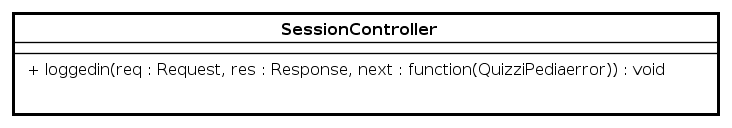
\includegraphics[scale=0.45]{UML/Classi/Back-End/QuizziPedia_Back-End_App_Controllers_Users_SessionController.png}
	\caption{QuizziPedia::Back-End::App::Controllers::Users::SessionController}
\end{figure}
\FloatBarrier
\begin{itemize}
	\item 
	\textbf{Descrizione}:\\
	Classe \textit{middleware\ped{G}} che, utilizzando \textit{Passport\ped{G}}, si occupa di controllare la consistenza dell'oggetto session durante la sessione associata all'utente autenticato. È un componente ConcreteHandler del design pattern \textit{Chain of responsibility\ped{G}};
	\item
	\textbf{Utilizzo}:\\
	Componente \textit{middleware\ped{G}} della catena, esegue controlli sullo stato della sessione relativa all'utente. Se l'utente non possiede i permessi adeguati o la sessione è scaduta restituisce un messaggio d'errore, altrimenti passa il controllo al prossimo ConcreteHandler che gestirà il normale flusso d'esecuzione del programma;
	\item
	\textbf{Relazioni con altre classi}:
	\begin{itemize}
		\item
		IN \texttt{UserController} \\
		Classe che raggruppa attraverso require i vari controllers responsabili delle operazioni legate alla gestione degli utenti. Si è scelto di predisporre questo raggruppamento per facilitare l'introduzione di nuove funzionalità legate alla gestione degli utenti;
		\item
		OUT \texttt{Session} \\
		Classe che gestisce la sessione utente dell'applicazione. Non sono stati modellati attributi e metodi di questa classe in quanto viene inizializzata da \textit{Express\ped{G}} ed utilizzata da \textit{Passport\ped{G}} attraverso funzionalità interne ai due \textit{middleware\ped{G}};
		\item
		OUT \texttt{UserModel} \\
		Classe che modella la creazione e la gestione dei dati utente.
	\end{itemize}
	\item
	\textbf{Metodi}:
	\begin{itemize}
		\item
		\texttt{+ loggedin(req: Request, res: Response, next: function(QuzziPediaError))} \\
		Metodo usato dal \textit{middleware\ped{G}} per verificare che l'utente che esegue una richiesta sia effettivamente un utente autenticato; \\
		\textbf{Parametri}:
		 \begin{itemize}
		  \item
			\texttt{req: Request} \\
			Rappresenta la richiesta inviata dal client;
		  \item
			\texttt{res: Response} \\
			Rappresenta la risposta che fornirà il server;
		  \item
		    \texttt{next: function(QuizziPediaError)} \\
			Rappresenta la \textit{callback\ped{G}} che il metodo deve chiamare al termine dell'elaborazione per passare il controllo ai successivi \textit{middleware\ped{G}}. La presenza del parametro facoltativo \texttt{QuizziPediaError} attiva la catena di gestione dell'errore in sostituzione della normale catena di gestione delle richieste.
		 \end{itemize}
	\end{itemize}	 
\end{itemize}	
\paragraph{QuizziPedia::Back-End::App::Controllers::Users::UserManagementController}
\label{QuizziPedia::Back-End::App::Controllers::Users::UserManagementController}
\begin{figure}[ht]
	\centering
	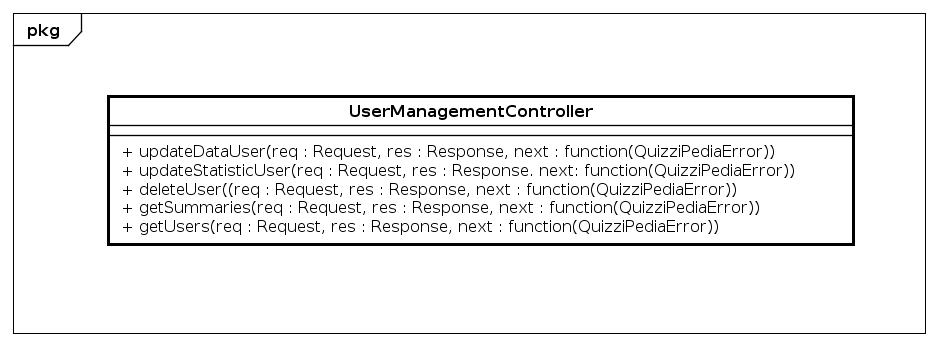
\includegraphics[scale=0.45]{UML/Classi/Back-End/QuizziPedia_Back-End_App_Controllers_Users_UserManagementController.png}
	\caption{QuizziPedia::Back-End::App::Controllers::Users::UserManagementController}
\end{figure}
\FloatBarrier
\begin{itemize}
	\item 
	\textbf{Descrizione}:\\
	Classe che gestisce la logica applicativa riguardante la visualizzazione e la modifica dei dati dell'utente.
Rappresenta il ConcreteHandler nel design pattern \textit{Chain of responsibility\ped{G}}. Utilizza \textit{Passport\ped{G}};
	\item
	\textbf{Utilizzo}:\\
	Viene utilizzata per gestire le richieste \textit{REST\ped{G}} legate agli utenti;
	\item
	\textbf{Relazioni con altre classi}:
	\begin{itemize}
		\item
		IN \texttt{UserController} \\
		Classe che raggruppa attraverso require i vari controllers responsabili delle operazioni legate alla gestione degli utenti. Si è scelto di predisporre questo raggruppamento per facilitare l'introduzione di nuove funzionalità legate alla gestione degli utenti;
		\item
		OUT \texttt{UserModel} \\
		Classe che modella la creazione e la gestione dei dati utente.
	\end{itemize}
	\item
	\textbf{Metodi}:
	\begin{itemize}
		\item
		\texttt{+ UpdatePasswordUser(req: Request, res: Response, next: function(QuzziPediaError))} \\
		Metodo usato dal \textit{middleware\ped{G}} per aggiorna la password dell'utente; \\
		\textbf{Parametri}:
		 \begin{itemize}
		  \item
			\texttt{req: Request} \\
			Rappresenta la richiesta inviata dal client;
		  \item
			\texttt{res: Response} \\
			Rappresenta la risposta che fornirà il server;
		  \item
		    \texttt{next: function(QuizziPediaError)} \\
			Rappresenta la \textit{callback\ped{G}} che il metodo deve chiamare al termine dell'elaborazione per passare il controllo ai successivi \textit{middleware\ped{G}}. La presenza del parametro facoltativo \texttt{QuizziPediaError} attiva la catena di gestione dell'errore in sostituzione della normale catena di gestione delle richieste.
		 \end{itemize}
		\item
		\texttt{+ UpdateDataUser(req: Request, res: Response, next: function(QuzziPediaError))} \\
		Metodo usato dal \textit{middleware\ped{G}} per aggiornare i dati dell'utente; \\
		\textbf{Parametri}:
		 \begin{itemize}
		  \item
			\texttt{req: Request} \\
			Rappresenta la richiesta inviata dal client;
		  \item
			\texttt{res: Response} \\
			Rappresenta la risposta che fornirà il server;
		  \item
		    \texttt{next: function(QuizziPediaError)} \\
			Rappresenta la \textit{callback\ped{G}} che il metodo deve chiamare al termine dell'elaborazione per passare il controllo ai successivi \textit{middleware\ped{G}}. La presenza del parametro facoltativo \texttt{QuizziPediaError} attiva la catena di gestione dell'errore in sostituzione della normale catena di gestione delle richieste.
		 \end{itemize}
		 \item
		\texttt{+ UpdateStatisticsUser(req: Request, res: Response, next: \\function(QuzziPediaError))} \\
		Metodo usato dal \textit{middleware\ped{G}} per aggiornare le statistiche dell'utente; \\
		\textbf{Parametri}:
		 \begin{itemize}
		  \item
			\texttt{req: Request} \\
			Rappresenta la richiesta inviata dal client;
		  \item
			\texttt{res: Response} \\
			Rappresenta la risposta che fornirà il server;
		  \item
		    \texttt{next: function(QuizziPediaError)} \\
			Rappresenta la \textit{callback\ped{G}} che il metodo deve chiamare al termine dell'elaborazione per passare il controllo ai successivi \textit{middleware\ped{G}}. La presenza del parametro facoltativo \texttt{QuizziPediaError} attiva la catena di gestione dell'errore in sostituzione della normale catena di gestione delle richieste.
		 \end{itemize}
		 \item
		 \texttt{+ deleteUser(req: Request, res: Response, next: function(QuzziPediaError))} \\
		Metodo usato dal \textit{middleware\ped{G}} per eliminare un utente dal sistema; \\
		\textbf{Parametri}:
		 \begin{itemize}
		  \item
			\texttt{req: Request} \\
			Rappresenta la richiesta inviata dal client;
		  \item
			\texttt{res: Response} \\
			Rappresenta la risposta che fornirà il server;
		  \item
		    \texttt{next: function(QuizziPediaError)} \\
			Rappresenta la \textit{callback\ped{G}} che il metodo deve chiamare al termine dell'elaborazione per passare il controllo ai successivi \textit{middleware\ped{G}}. La presenza del parametro facoltativo \texttt{QuizziPediaError} attiva la catena di gestione dell'errore in sostituzione della normale catena di gestione delle richieste.
		 \end{itemize}
		  \item
		 \texttt{+ getInfo(req: Request, res: Response, next: function(QuzziPediaError))} \\
		Metodo usato dal \textit{middleware\ped{G}} per ottenere le informazioni dell'utente; \\
		\textbf{Parametri}:
		 \begin{itemize}
		  \item
			\texttt{req: Request} \\
			Rappresenta la richiesta inviata dal client;
		  \item
			\texttt{res: Response} \\
			Rappresenta la risposta che fornirà il server;
		  \item
		    \texttt{next: function(QuizziPediaError)} \\
			Rappresenta la \textit{callback\ped{G}} che il metodo deve chiamare al termine dell'elaborazione per passare il controllo ai successivi \textit{middleware\ped{G}}. La presenza del parametro facoltativo \texttt{QuizziPediaError} attiva la catena di gestione dell'errore in sostituzione della normale catena di gestione delle richieste.
		 \end{itemize}
		  \item
		 \texttt{+ getStatistics(req: Request, res: Response, next: function(QuzziPediaError))} \\
		Metodo usato dal \textit{middleware\ped{G}} per ottenere le statistiche dell'utente; \\
		\textbf{Parametri}:
		 \begin{itemize}
		  \item
			\texttt{req: Request} \\
			Rappresenta la richiesta inviata dal client;
		  \item
			\texttt{res: Response} \\
			Rappresenta la risposta che fornirà il server;
		  \item
		    \texttt{next: function(QuizziPediaError)} \\
			Rappresenta la \textit{callback\ped{G}} che il metodo deve chiamare al termine dell'elaborazione per passare il controllo ai successivi \textit{middleware\ped{G}}. La presenza del parametro facoltativo \texttt{QuizziPediaError} attiva la catena di gestione dell'errore in sostituzione della normale catena di gestione delle richieste.
		 \end{itemize}
		   \item
		 \texttt{+ getSummary(req: Request, res: Response, next: function(QuzziPediaError))} \\
		Metodo usato dal \textit{middleware\ped{G}} per ottenere il riepilogo di un determinato questionario svolto; \\
		\textbf{Parametri}:
		 \begin{itemize}
		  \item
			\texttt{req: Request} \\
			Rappresenta la richiesta inviata dal client;
		  \item
			\texttt{res: Response} \\
			Rappresenta la risposta che fornirà il server;
		  \item
		    \texttt{next: function(QuizziPediaError)} \\
			Rappresenta la \textit{callback\ped{G}} che il metodo deve chiamare al termine dell'elaborazione per passare il controllo ai successivi \textit{middleware\ped{G}}. La presenza del parametro facoltativo \texttt{QuizziPediaError} attiva la catena di gestione dell'errore in sostituzione della normale catena di gestione delle richieste.
		 \end{itemize}
		 \item
		  \texttt{+ getSummaries(req: Request, res: Response, next: function(QuzziPediaError))} \\
		Metodo usato dal \textit{middleware\ped{G}} per ottenere la cronologia dei questionari svolti dall'utente; \\
		\textbf{Parametri}:
		 \begin{itemize}
		  \item
			\texttt{req: Request} \\
			Rappresenta la richiesta inviata dal client;
		  \item
			\texttt{res: Response} \\
			Rappresenta la risposta che fornirà il server;
		  \item
		    \texttt{next: function(QuizziPediaError)} \\
			Rappresenta la callback che il metodo deve chiamare al termine dell'elaborazione per passare il controllo ai successivi \textit{middleware\ped{G}}. La presenza del parametro facoltativo \texttt{QuizziPediaError} attiva la catena di gestione dell'errore in sostituzione della normale catena di gestione delle richieste.
		 \end{itemize}
		  \item
		 	 \texttt{+ getUsers(req: Request, res: Response, next: function(QuzziPediaError))} \\
		Metodo usato dal \textit{middleware\ped{G}} per ottenere i dati dei vari utenti; \\
		\textbf{Parametri}:
		 \begin{itemize}
		  \item
			\texttt{req: Request} \\
			Rappresenta la richiesta inviata dal client;
		  \item
			\texttt{res: Response} \\
			Rappresenta la risposta che fornirà il server;
		  \item
		    \texttt{next: function(QuizziPediaError)} \\
			Rappresenta la \textit{callback\ped{G}} che il metodo deve chiamare al termine dell'elaborazione per passare il controllo ai successivi \textit{middleware\ped{G}}. La presenza del parametro facoltativo \texttt{QuizziPediaError} attiva la catena di gestione dell'errore in sostituzione della normale catena di gestione delle richieste.
		 \end{itemize}
	\end{itemize}	 
\end{itemize}
